\chapter{Interfaccia web di amministrazione}\label{capitolo5}
Al fine di ospitare la pagina web che contiene il pannello di amministrazione \`e necessario
creare una nuova classe server oltre a quella gi\`a esistente, citata nel capitolo \ref{cap:MMalto}.
Il server gira su una porta differente rispetto al primo, indicata nel file di configurazione del MM,
ed inoltre \`e accessibile da qualsiasi utente all'interno della sottorete.
La struttura del server viene gestita con Express, spiegato nel capitolo \ref{cap:express}, che offre funzioni per gestire
pi\`u facilmente le richieste delle pagine e relative risposte.
Inoltre all'inizializzazione del server viene passato come parametro il file di configurazione del
MM.
Affinch\`e l'interfaccia funzioni completamente \`e stato necessario inserire una nuova dipendenza:
per ogni modulo deve essere creato un file JSON con lo stesso nome,
contenente i campi e le variabili della propria configurazione.
In questo capitolo vengono trattati le metodologie per l'individuazione dei moduli
presenti nel MM con i relativi file JSON per poterli inserire in un men\`u laterale del
pannello di configurazione, come questi vengano mostrati e poi spediti
al server in seguito ad una modifica \ref{cap:individuazione}.\\[1\baselineskip]

\section{Individuazione e visualizzazione dei moduli nell'interfaccia}\label{cap:individuazione}
Come gi\`a trattato nel capitolo \ref{cap:app} tutti i moduli sono contenuti nella
cartella \textit{Modules} del MM. Il server, tramite una funzione della libreria \textit{fs} (File System),
legge i nomi di tutte le cartelle contenute all'interno di \textit{Modules} il cui percorso \`e stato passato
come parametro alla funzione. In seguito, salva tutti i nomi dei moduli
in una lista, filtrando i file e le cartelle che non si riferisocno ad essi.
La funzione per leggere le directory di \textit{fs} offre un metodo per leggere ed elencare le cartelle in
modo sincrono, cos\`i da non rendere necessario l'utilizzo di callback.\\
All'interno di \textit{Modules} \`e presente una cartella \textit{default}, che contiene
i moduli standard in dotazione con il MM. Per poter elencare anche questi ultimi \`e stato necessario utilizzare la funzione
della libreria \textit{fs} anche su quest'ultima cartella e concatenare, successivamente, le due liste,
per ottenere un'unica lista con tutti i moduli, necessaria per poter popolare il men\`u del pannello web di configurazione.\\
Tutte le pagine web che ritorna il server sono divise in 2 sezioni come illustrato nella figura \ref{fig:interfaccia}:
\begin{itemize}
\item Il men\`u laterale, che contiene tutti i moduli precedentemente cercati. Ogni modulo corrisponde ad un'opzione che permette di fare richiesta di una pagina
contenente la configurazione del modulo selezionato.
\item Le varie impostazioni del modulo, visualizzate tramite \textit{CodeMirror}\cite{CodeMirror}, una componente Javascript
che permette l'implementazione di un'area di testo per la modifica di codici all'interno di una pagina web.\\[1\baselineskip]
\end{itemize}
Una pagina web consiste in un file con estensione \textit{mustache} che contiene
codici HTML e variabili mustache, motore di template esposto nella sezione \ref{cap:mustache} tutto ci\`o rappresenta lo
scheletro della pagina usato per ogni modulo.
Il server, alla richiesta di una pagina di uno specifico modulo, ricerca il relativo file JSON all'interno della cartella del modulo stesso e lo
passa come parametro sottoforma di oggetto JSON alla funzione \textit{render}, necessaria per la creazione e visualizzazione della pagina.
Insieme vengono passati i parametri \textit{posizione} ed \textit{header}, trattati nel capitolo \ref{cap:MMconf}, estratti dal file
di configurazione passato all'inizializzazione del server.
Durante la creazione della pagina, i vari campi passati come parametro, vengono inseriti dentro l'area di testo di \textit{CodeMirror}, che permetter\`a di eseguirne
le modifiche. Sotto all'area di testo \`e presente un bottone, che permette di attivare o disattivare il modulo nel MM; tuttavia affinch\`e la modifica
venga apportata \`e richiesto un riavvio del software. Le modifiche apportate vengono spedite al server che si occupa di salvarle nel file di configurazione
principale del MM.

\begin{figure}[H]
    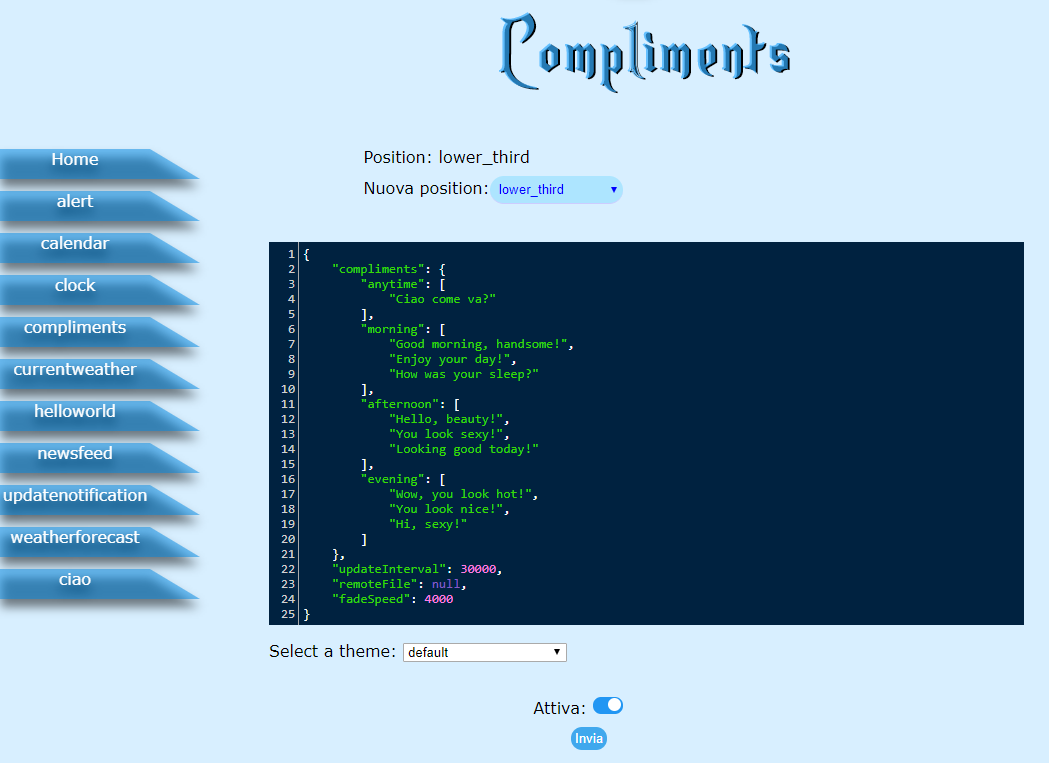
\includegraphics[width=1\textwidth, height=0.5\textheight]{interfacciamm}
    \caption{Interfaccia web di amminsitrazione}
    \label{fig:interfaccia}
\end{figure}
